



\bta{2008}




\section{Use of English}

\noindent
\textbf{Directions:}\\
Read the following text. Choose the best word (s) for each
	numbered blank and mark A, B, C or D on ANSWER
	SHEET 1. (10 points)
	
	
\TiGanSpace	
	

The idea that some groups of people may be more intelligent than others
is one of those hypotheses that dare not speak its name. But Gregory
Cochran is \cloze to say it anyway. He is
that \cloze bird, a scientist who works
independently \cloze any institution. He helped popularize the
idea that some diseases not \cloze thought to have a bacterial
cause were actually infections, which aroused much controversy when it
was first suggested.

\cloze he, however, might tremble at the \cloze of what he
is about to do. Together with another two scientists, he is publishing a
paper which not only \cloze that one group of humanity is more
intelligent than the others, but explains the process that has brought
this about. The group in \cloze are a particular people originated
from central Europe. The process is natural selection.

This group generally do well in IQ test, \cloze 12-15 points
above the \cloze value of 100, and have
contributed \cloze to the intellectual and cultural life of the
West, as the \cloze of their elites, including several
world-renowned scientists, \cloze. They also suffer more often
than most people from a number of nasty genetic diseases, such as breast
cancer. These facts, \cloze , have previously been thought
unrelated. The former has been \cloze to social effects, such as
a strong tradition of \cloze education. The latter was seen as a(an) \cloze of genetic isolation. Dr. Cochran suggests that the
intelligence and diseases are intimately \cloze. His argument
is that the unusual history of these people has \cloze them to
unique evolutionary pressures that have resulted in
this \cloze state of affairs.



\newpage

\begin{enumerate}
	%\renewcommand{\labelenumi}{\arabic{enumi}.}
	% A(\Alph) a(\alph) I(\Roman) i(\roman) 1(\arabic)
	%设定全局标号series=example	%引用全局变量resume=example
	%[topsep=-0.3em,parsep=-0.3em,itemsep=-0.3em,partopsep=-0.3em]
	%可使用leftmargin调整列表环境左边的空白长度 [leftmargin=0em]
	\item


\fourchoices
{selected}
{prepared}
{obliged}
{pleased}




\item


\fourchoices
{unique}
{particular}
{special}
{rare}




\item


\fourchoices
{of}
{with}
{in}
{against}




\item

\fourchoices
{subsequently}
{presently}
{previously}
{lately}




\item


\fourchoices
{Only}
{So}
{Even}
{Hence}




\item


\fourchoices
{thought}
{sight}
{cost}
{risk}




\item


\fourchoices
{advises}
{suggests}
{protests}
{objects}




\item


\fourchoices
{progress}
{fact}
{need}
{question}




\item


\fourchoices
{attaining}
{scoring}
{reaching}
{calculating}




\item


\fourchoices
{normal}
{common}
{mean}
{total}




\item

\fourchoices
{unconsciously}
{disproportionately}
{indefinitely}
{unaccountably}




\item


\fourchoices
{missions}
{fortunes}
{interests}
{careers}




\item


\fourchoices
{affirm}
{witness}
{observe}
{approve}




\item


\fourchoices
{moreover}
{therefore}
{however}
{meanwhile}




\item


\fourchoices
{given up}
{got over}
{carried on}
{put down}




\item

\fourchoices
{assessing}
{supervising}
{administering}
{valuing}




\item

\fourchoices
{development}
{origin}
{consequence}
{instrument}



\item


\fourchoices
{linked}
{integrated}
{woven}
{combined}




\item


\fourchoices
{limited}
{subjected}
{converted}
{directed}




\item

\fourchoices
{paradoxical}
{incompatible}
{inevitable}
{continuous}


	
\end{enumerate}


\vfil

\section{Reading Comprehension}




\noindent
\textbf{Part A}\\
\textbf{Directions:}\\
Read the following four texts. Answer the questions below each
text by choosing A, B, C or
D. Mark your answers
on ANSWER SHEET 1. (40 points)


\newpage
\subsection{Text 1}


While still catching up to men in some spheres of modern life, women
appear to be way ahead in at least one undesirable category. ``Women are
particularly susceptible to developing depression and anxiety disorders
in response to stress compared to men,'' according to Dr. Yehuda, chief
psychiatrist at New York's Veteran's Administration Hospital.

Studies of both animals and humans have shown that sex hormones somehow
affect the stress response, causing females under stress to produce more
of the trigger chemicals than do males under the same conditions. In
several of the studies, when stressed-out female rats had their ovaries
(the female reproductive organs) removed, their chemical responses
became equal to those of the males.

Adding to a woman's increased dose of stress chemicals, are her
increased ``opportunities'' for stress. ``It's not necessarily that
women don't cope as well. It's just that they have so much more to cope
with,'' says Dr. Yehuda. ``Their capacity for tolerating stress may even
be greater than men's,'' she observes, ``it's just that they're dealing
with so many more things that they become worn out from it more visibly
and sooner.''

Dr. Yehuda notes another difference between the sexes. ``I think that
the kinds of things that women are exposed to tend to be in more of a
chronic or repeated nature. Men go to war and are exposed to combat
stress. Men are exposed to more acts of random physical violence. The
kinds of interpersonal violence that women are exposed to tend to be in
domestic situations, by, unfortunately, parents or other family members,
and they tend not to be one-shot deals. The wear-and-tear that comes
from these longer relationships can be quite devastating.''

Adeline Alvarez married at 18 and gave birth to a son, but was
determined to finish college. ``I struggled a lot to get the college
degree. I was living in so much frustration that that was my escape, to
go to school, and get ahead and do better.'' Later, her marriage ended
and she became a single mother. ``It's the hardest thing to take care of
a teenager, have a job, pay the rent, pay the car payment, and pay the
debt. \uline{I lived from paycheck to paycheck}.''

Not everyone experiences the kinds of severe chronic stresses Alvarez
describes. But most women today are coping with a lot of obligations,
with few breaks, and feeling the strain. Alvarez's experience
demonstrates the importance of finding ways to diffuse stress before it
threatens your health and your ability to function.


\begin{enumerate}[resume]
	%\renewcommand{\labelenumi}{\arabic{enumi}.}
	% A(\Alph) a(\alph) I(\Roman) i(\roman) 1(\arabic)
	%设定全局标号series=example	%引用全局变量resume=example
	%[topsep=-0.3em,parsep=-0.3em,itemsep=-0.3em,partopsep=-0.3em]
	%可使用leftmargin调整列表环境左边的空白长度 [leftmargin=0em]
	\item
 Which of the following is true according to the first two
paragraphs?


A. Women are biologically more vulnerable to stress.


B. Women are still suffering much stress caused by men.


C. Women are more experienced than men in coping with stress.


D. Men and women show different inclinations when faced with
stress.



\item
 Dr. Yehuda's research suggests that women \lineread.


\fourchoices
{need extra doses of chemicals to handle stress}
{have limited capacity for tolerating stress}
{are more capable of avoiding stress}
{are exposed to more stress}




\item
According to Paragraph 4, the stress women confront tends to
be \lineread.


\fourchoices
{domestic and temporary}
{irregular and violent}
{durable and frequent}
{trivial and random}


\item
 The sentence ``I lived from paycheck to paycheck.'' (Line 5,
Para. 5) shows that \lineread.


\fourchoices
{Alvarez cared about nothing but making money}
{Alvarez's salary barely covered her household expenses}
{Alvarez got paychecks from different jobs}
{Alvarez paid practically everything by check}



\item
Which of the following would be the best title for the
text?


\fourchoices
{Strain of Stress: No Way Out?}
{Response to Stress: Gender Difference}
{Stress Analysis: What Chemicals Say?}
{Gender Inequality: Women Under Stress}

\end{enumerate}



\newpage
\subsection{Text 2}


It used to be so straightforward. A team of researchers working together
in the laboratory would submit the results of their research to a
journal. A journal editor would then remove the author's names and
affiliations from the paper and send it to their peers for review.
Depending on the comments received, the editor would accept the paper
for publication or decline it. Copyright rested with the journal
publisher, and researchers seeking knowledge of the results would have
to subscribe to the journal.

No longer. The Internet---and pressure from funding agencies, who are
questioning why commercial publishers are making money from
government--funded research by restricting access to it---is making
access to scientific results a reality. The Organization for Economic
Co-operation and Development (OECD) has just issued a report describing
the far-reaching consequences of this. The report, by John Houghton of
Victoria University in Australia and Graham Vickery of the OECD, makes
heavy reading for publishers who have, so far, made handsome profits.
But it goes further than that. It signals a change in what has, until
now, been a key element of scientific endeavor.

The value of knowledge and the return on the public investment in
research depends, in part, upon wide distribution and ready access. It
is big business. In America, the core scientific publishing market is
estimated at between \$7 billion and \$11 billion. The International
Association of Scientific, Technical and Medical Publishers says that
there are more than 2, 000 publishers worldwide specializing in these
subjects. They publish more than 1.2 million articles each year in some
16, 000 journals.

This is now changing. According to the OECD report, some 75\% of
scholarly journals are now online. Entirely new business models are
emerging; three main ones were identified by the report's authors. There
is the so-called big deal, where institutional subscribers pay for
access to a collection of online journal titles through site-licensing
agreements. There is open-access publishing, typically supported by
asking the author (orhis employer) to pay for the paper to be published.
Finally, there are open-access archives, where organizations such as
universities or international laboratories support institutional
repositories. Other models exist that are hybrids of these three, such
as delayed open-access, where journals allow only subscribers to read a
paper for the first six months, before making it freely available to
everyone who wishes to see it. All this could change the traditional
form of the peer-review process, at least for the publication of papers.

\begin{enumerate}[resume]
	%\renewcommand{\labelenumi}{\arabic{enumi}.}
	% A(\Alph) a(\alph) I(\Roman) i(\roman) 1(\arabic)
	%设定全局标号series=example	%引用全局变量resume=example
	%[topsep=-0.3em,parsep=-0.3em,itemsep=-0.3em,partopsep=-0.3em]
	%可使用leftmargin调整列表环境左边的空白长度 [leftmargin=0em]
	\item
In the first paragraph, the author discusses \lineread.


\fourchoices
{the background information of journal editing}
{the publication routine of laboratory reports}
{the relations of authors with journal publishers}
{the traditional process of journal publication}



\item
Which of the following is true of the OECD report?


\fourchoices
{It criticizes government-funded research.}
{It introduces an effective means of publication.}
{It upsets profit-making journal publishers.}
{It benefits scientific research considerably.}



\item
According to the text, online publication is significant in
that \lineread.


\fourchoices
{it provides an easier access to scientific results}
{it brings huge profits to scientific researchers}
{it emphasizes the crucial role of scientific knowledge}
{it facilitates public investment in scientific research}



\item
With the open-access publishing model, the author of a paper
is required to \lineread.


\fourchoices
{cover the cost of its publication}
{subscribe to the journal publishing it}
{allow other online journals to use it freely}
{complete the peer-review before submission}



\item
 Which of the following best summarizes the text?


\fourchoices
{The Internet is posing a threat to publishers.}
{A new mode of publication is emerging.}
{Authors welcome the new channel for publication.}
{Publication is rendered easily by online service.}


	
\end{enumerate}


\newpage
\subsection{Text 3}


In the early 1960s Wilt Chamberlain was one of the only three players in
the National Basketball Association (NBA) listed at over seven feet. If
he had played last season, however, he would have been one of 42. The
bodies playing major professional sports have changed dramatically over
the years, and managers have been more than willing to adjust team
uniforms to fit the growing numbers of bigger, longer frames.

The trend in sports, though, may be obscuring an unrecognized reality:
Americans have generally stopped growing. Though typically about two
inches taller now than 140 years ago, today's people---especially those
born to families who have lived in the U.S. for many
generations---apparently reached their limit in the early 1960 s. And they
aren't likely to get any taller. ``In the general population today, at
this genetic, environmental level, we've pretty much gone as far as we
can go,'' says anthropologist William Cameron Chumlea of Wright State
University. In the case of NBA players, their increase in height appears
to result from the increasingly common practice of recruiting players
from all over the world.

Growth, which rarely continues beyond the age of 20, demands calories
and nutrients---notably, protein---to feed expanding tissues. At the
start of the 20th century, under-nutrition and childhood infections got
in the way. But as diet and health improved, children and adolescents
have, on average, increased in height by about an inch and a half every
20 years, a pattern known as the secular trend in height. Yet according
to the Centers for Disease Control and Prevention, average height---5'9"
for men, 5'4" for women---hasn't really changed since 1960.

Genetically speaking, there are advantages to avoiding substantial
height. During childbirth, larger babies have more difficulty passing
through the birth canal. Moreover, even though humans have been upright
for millions of years, our feet and back continue to struggle with
bipedal posture and cannot easily withstand repeated strain imposed by
oversize limbs. ``There are some real constraints that are set by the
genetic architecture of the individual organism,'' says anthropologist
William Leonard of Northwestern University.

Genetic maximums can change, but don't expect this to happen soon.
Claire
C. Gordon, senior anthropologist at the Army Research Center in
Natick, Mass., ensures that 90 percent of the uniforms and workstations
fit recruits without alteration. She says that, unlike those for
basketball, the length of military uniforms has not changed for some
time. And if you need to predict human height in the near future to
design a piece of equipment, Gordon says that by and large, ``you could
use today's data and feel fairly confident.''


\begin{enumerate}[resume]
	%\renewcommand{\labelenumi}{\arabic{enumi}.}
	% A(\Alph) a(\alph) I(\Roman) i(\roman) 1(\arabic)
	%设定全局标号series=example	%引用全局变量resume=example
	%[topsep=-0.3em,parsep=-0.3em,itemsep=-0.3em,partopsep=-0.3em]
	%可使用leftmargin调整列表环境左边的空白长度 [leftmargin=0em]
	\item
Wilt Chamberlain is cited as an example to \lineread.


\fourchoices
{illustrate the change of height of NBA players}
{show the popularity of NBA players in the U.S.}
{compare different generations of NBA players}
{assess the achievements of famous NBA players}



\item
Which of the following plays a key role in body growth
according to the text?


\fourchoices
{Genetic modification.}
{Natural environment.}
{Living standards.}
{Daily exercise.}



\item
 On which of the following statements would the author most
probably agree?


\fourchoices
{Non-Americans add to the average height of the nation.}
{Human height is conditioned by the upright posture.}
{Americans are the tallest on average in the world.}
{Larger babies tend to become taller in adulthood.}


\item
 We learn from the last paragraph that in the near future \lineread.


\fourchoices
{the garment industry will reconsider the uniform size}
{the design of military uniforms will remain unchanged}
{genetic testing will be employed in selecting sportsmen}
{the existing data of human height will still be applicable}



\item
The text intends to tell us that \lineread.


\fourchoices
{the change of human height follows a cyclic pattern}
{human height is becoming even more predictable}
{Americans have reached their genetic growth limit}
{the genetic pattern of Americans has altered}

\end{enumerate}


\newpage
\subsection{Text 4}


In 1784, five years before he became president of the United States,
George Washington, 52, was nearly toothless. So he hired a dentist to
transplant nine teeth into his jaw---having extracted them from the
mouths of his slaves.

That's a far different image from the cherry-tree-chopping George most
people remember from their history books. But recently, many historians
have begun to focus on the role slavery played in the lives of the
founding generation. They have been spurred in part by DNA evidence made
available in 1998, which almost certainly proved Thomas Jefferson had
fathered at least one child with his slave Sally Hemings. And only over
the past 30 years have scholars examined history from the bottom up.
Works of several historians reveal the moral compromises made by the
nation's early leaders and the fragile nature of the country's infancy.
More significantly, they argue that many of the Founding Fathers knew
slavery was wrong---and yet most did little to fight it.

More than anything, the historians say, the founders were hampered by
the culture of their time. While Washington and Jefferson privately
expressed distaste for slavery, they also understood that it was part of
the political and economic bedrock of the country they helped to create.

For one thing, the South could not afford to part with its slaves.
Owning slaves was ``like having a large bank account,'' says Wiencek,
author of \emph{An Imperfect God: George Washington, His Slaves, and the
Creation of America}. The southern states would not have signed the
Constitution without protections for the ``peculiar institution,''
including a clause that counted a slave as three fifths of a man for
purposes of congressional representation.

And the statesmen's political lives depended on slavery. The
three-fifths formula handed Jefferson his narrow victory in the
presidential election of 1800 by inflating the votes of the southern
states in the Electoral College. Once in office, Jefferson extended
slavery with the Louisiana Purchase in 1803; the new land was carved
into 13 states, including three slave states.

Still, Jefferson freed Hemings's children---though not Hemings herself
or his approximately 150 other slaves. Washington, who had begun to
believe that all men were created equal after observing the
bravery of the black soldiers during the Revolutionary War, overcame the
strong opposition of his relatives to grant his slaves their freedom in
his will. Only a decade earlier, such an act would have required
legislative approval in Virginia.

\begin{enumerate}[resume]
	%\renewcommand{\labelenumi}{\arabic{enumi}.}
	% A(\Alph) a(\alph) I(\Roman) i(\roman) 1(\arabic)
	%设定全局标号series=example	%引用全局变量resume=example
	%[topsep=-0.3em,parsep=-0.3em,itemsep=-0.3em,partopsep=-0.3em]
	%可使用leftmargin调整列表环境左边的空白长度 [leftmargin=0em]
	\item
George Washington's dental surgery is mentioned to \lineread.


\fourchoices
{show the primitive medical practice in the past}
{demonstrate the cruelty of slavery in his days}
{stress the role of slaves in the U.S. history}
{reveal some unknown aspect of his life}



\item
We may infer from the second paragraph that \lineread.


\fourchoices
{DNA technology has been widely applied to history research}
{in its early days the U.S. was confronted with delicate situations}
{historians deliberately made up some stories of Jefferson's life}
{political compromises are easily found throughout the U.S. history}



\item
What do we learn about Thomas Jefferson?


\fourchoices
{His political view changed his attitude towards slavery.}
{His status as a father made him free the child slaves.}
{His attitude towards slavery was complex.}
{His affair with a slave stained his prestige.}


\item
Which of the following is true according to the text?


\fourchoices
{Some Founding Fathers benefit politically from slavery.}
{Slaves in the old days did not have the right to vote.}
{Slave owners usually had large savings accounts.}
{Slavery was regarded as a peculiar institution.}


\item
Washington's decision to free slaves originated from his \lineread.


\fourchoices
{moral considerations}
{military experience}
{financial conditions}
{political stand}


\end{enumerate}


\newpage

\noindent
\textbf{Part B}\\
\textbf{Directions:}\\
In the following text, some segments have been removed. For
Questions 41-45, choose the most suitable one from the list A-G to fit
into each of the numbered blanks. There are two extra choices, which do
not fit in any of the blanks. Mark your answers on ANSWER SHEET 1. (10
points)


\TiGanSpace


The time for sharpening pencils, arranging your desk, and doing almost
anything else instead of writing has ended. The first draft will appear
on the page only if you stop avoiding the inevitable and sit, stand up,
or lie down to write. \linefill.

Be flexible. Your outline should smoothly conduct you from one point to
the next, but do not permit it to railroad you. If a relevant and
important idea occurs to you now, work it into the draft. \linefill. Grammar, punctuation, and spelling can
wait until you revise. Concentrate on what you are saying. Good writing
most often occurs when you are in hot pursuit of an idea rather than in
a nervous search for errors.

\linefill. Your pages will be easier to keep
track of that way, and, if you have to clip a paragraph to place it
elsewhere, you will not lose any writing on other side.

If you are working on a word processor, you can take advantage of its
capacity to make additions and deletions as well as move entire
paragraphs by making just a few simple keyboard commands. Some software
programs can also check spelling and certain grammatical elements in
your writing. \linefill. These printouts are
also easier to read than the screen when you work on revisions.

Once you have a first draft on paper, you can delete material that is
unrelated to your thesis and add material necessary to illustrate your
points and make your paper convincing. The student who wrote ``The A\&P
as a State of Mind'' wisely dropped a paragraph that questioned whether
Sammy displays chauvinistic attitudes toward women. \linefill.

Remember that your initial draft is only that. You should go through the
paper many times---and then again---working to substantiate and clarify
your ideas. You may even end up with several entire versions of the
paper. Rewrite. The sentences within each paragraph should be related to
a single topic. Transitions should connect one paragraph to the next so
that there are no abrupt or confusing shifts. Awkward or wordy phrasing
or unclear sentences and paragraphs should be mercilessly poked and
prodded into shape.



\begin{listmatch}
	%\renewcommand{\labelenumi}{\arabic{enumi}.}
	% A(\Alph) a(\alph) I(\Roman) i(\roman) 1(\arabic)
	%设定全局标号series=example	%引用全局变量resume=example
	%[topsep=-0.3em,parsep=-0.3em,itemsep=-0.3em,partopsep=-0.3em]
	%可使用leftmargin调整列表环境左边的空白长度 [leftmargin=0em]
	\item
To make revising easier, leave wide margins and extra space
between lines so that you can easily add words, sentences and
corrections. Write on only one side of the paper.


\item 
After you have clearly and adequately developed the body of your
paper, pay particular attention to the introductory and concluding
paragraphs. It's probably best to write the introduction last, after you
know precisely what you are introducing. Concluding paragraphs demand
equal attention because they leave the reader with a final impression.


\item 
 It's worth remembering, however, that though a clean copy fresh
off a printer may look terrific, it will read only as well as the
thinking and writing that have gone into it. Many writers prudently
store their data on disks and print their pages each time they finish a
draft to avoid losing any material because of power failures or other
problems.


\item 
 It makes no difference how you write, just so you do. Now that
you have developed a topic into a tentative thesis, you can assemble
your notes and begin to flesh out whatever outline you have made.


\item 
Although this is an interesting issue, it has nothing to do with
the thesis, which explains how the setting influences Sammy's decision
to quit his job. Instead of including that paragraph, she added one that
described Lengel's crabbed response to the girls so that she could lead
up to the A\&P ``policy'' he enforces.


\item 
 In the final paragraph about the significance of the setting in
``A\&P'' the student brings together the reasons Sammy quit his job by
referring to his refusal to accept Lengel's store policies.


\item 
By using the first draft as a means of thinking about what you
want to say, you will very likely discover more than your notes
originally suggested. Plenty of good writers don't use outlines at all
but discover ordering principles as they write. Do not attempt to
compose a perfectly correct draft the first time around.

\end{listmatch}




\noindent
\textbf{Part C}\\
\textbf{Directions:}\\
Read the following text carefully and then translate the
underlined segments into Chinese. Your translation should be written
neatly on \textbf{ANSWER SHEET 2}. (10 points)



\TiGanSpace


In his autobiography, Darwin himself speaks of his intellectualpowers
with extraordinary modesty. He points out that he always experienced
much difficulty in expressing himself clearly and concisely, but
\transnum \uline{he believes that this very difficulty may have had the
compensating advantage of forcing him to think long and intently about
every sentence, and thus enabling him to detect errors in reasoning and
in his own observations}. He disclaimed the possession of any great
quickness of apprehension or wit, such as distinguished Huxley.
\transnum \uline{He asserted, also, that his power to follow a long and
purely abstract train of thought was very limited, for which reason he
felt certain that he never could have succeeded with mathematics}. His
memory, too, he described as extensive, but hazy. So poor in one sense
was it that he never could remember for more than a few days a single
date or a line of poetry. \transnum \uline{On the other hand, he did not
accept as well founded the charge made by some of his critics that,
while he was a good observer, he had no power of reasoning}. This, he
thought, could not be true, because the ``Origin of Species'' is one
long argument from the beginning to the end, and has convinced many able
men. No one, he submits, could have written it without possessing some
power of reasoning. He was willing to assert that ``I have a fair share
of invention, and of common sense or judgment, such as every fairly
successful lawyer or doctor must have, but not, I believe, in any higher
degree.'' \transnum \uline{He adds humbly that perhaps he was ``superior
to the common run of men in noticing things which easily escape
attention, and in observing them carefully}.''

Writing in the last year of his life, he expressed the opinion that in
two or three respects his mind had changed during the preceding twenty
or thirty years. Up to the age of thirty or beyond it poetry of many
kinds gave him great pleasure. Formerly, too, pictures had given him
considerable, and music very great, delight. In 1881, however, he said:
``Now for many years I cannot endure to read a line of poetry. I have
also almost lost my taste for pictures or music.''
\transnum \uline{Darwin} \uline{was convinced that the loss of these
tastes was not only a loss of happiness, but might possibly be injurious
to the intellect, and more probably to the moral character}.


\newpage

\section{Writing}


\noindent
\textbf{Part A}\\
\textbf{51. Directions:}

You have just come back from Canada and found a music CD
in your luggage that you forgot to return to Bob, your landlord there.
Write him a letter to
\begin{listwrite}
	%\renewcommand{\labelenumi}{\arabic{enumi}.}
	% A(\Alph) a(\alph) I(\Roman) i(\roman) 1(\arabic)
	%设定全局标号series=example	%引用全局变量resume=example
	%[topsep=-0.3em,parsep=-0.3em,itemsep=-0.3em,partopsep=-0.3em]
	%可使用leftmargin调整列表环境左边的空白长度 [leftmargin=0em]
	\item
 make an apology, and

\item 
suggest a solution.
\end{listwrite}

You should write about 100 words on ANSWER SHEET 2.

\textbf{Do not} sign your own name at the end of the letter. Use ``Li
Ming'' instead.

\textbf{Do not} write the address. (10 points)

\vspace{2em}


\noindent
\textbf{Part B}\\
\textbf{52. Directions:}

Write an essay of 160-200 words based on the following drawing. In your
essay, you should
\begin{listwrite}
	%\renewcommand{\labelenumi}{\arabic{enumi}.}
	% A(\Alph) a(\alph) I(\Roman) i(\roman) 1(\arabic)
	%设定全局标号series=example	%引用全局变量resume=example
	%[topsep=-0.3em,parsep=-0.3em,itemsep=-0.3em,partopsep=-0.3em]
	%可使用leftmargin调整列表环境左边的空白长度 [leftmargin=0em]
	\item
 describe the drawing briefly,

\item 
explain its intended meaning, and then

\item 
give your comments.
\end{listwrite}

You should write neatly on ANSHWER SHEET 2. (20 points)



\begin{figure}[h!]
	\centering
	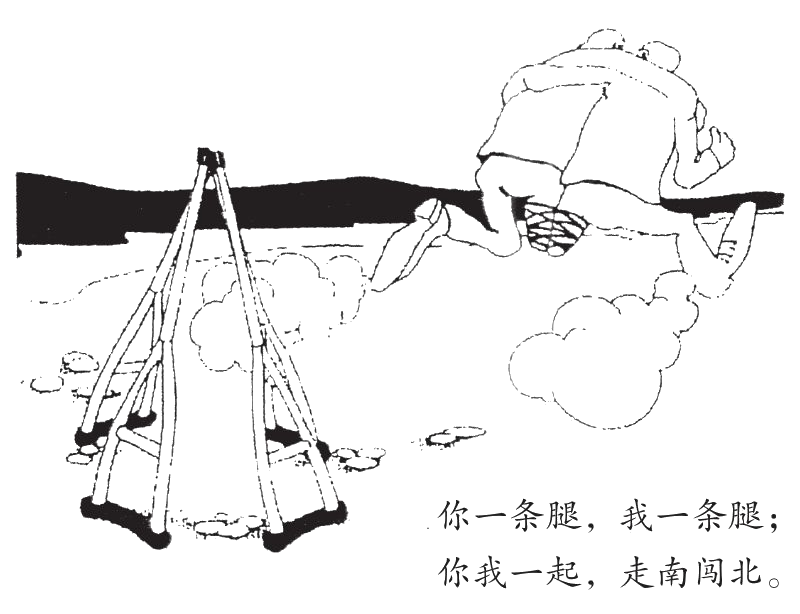
\includegraphics[width=0.54\linewidth]{picture/2008.png}
\end{figure}

